\documentclass{minimal}
\usepackage{amsmath}
\usepackage[T1]{fontenc}
\usepackage[utf8]{inputenc}

\usepackage{tikz}
\usetikzlibrary{arrows, shapes, matrix}
%\usetikzlibrary{external}
%\tikzexternalize[prefix=tikz/]

\begin{document}

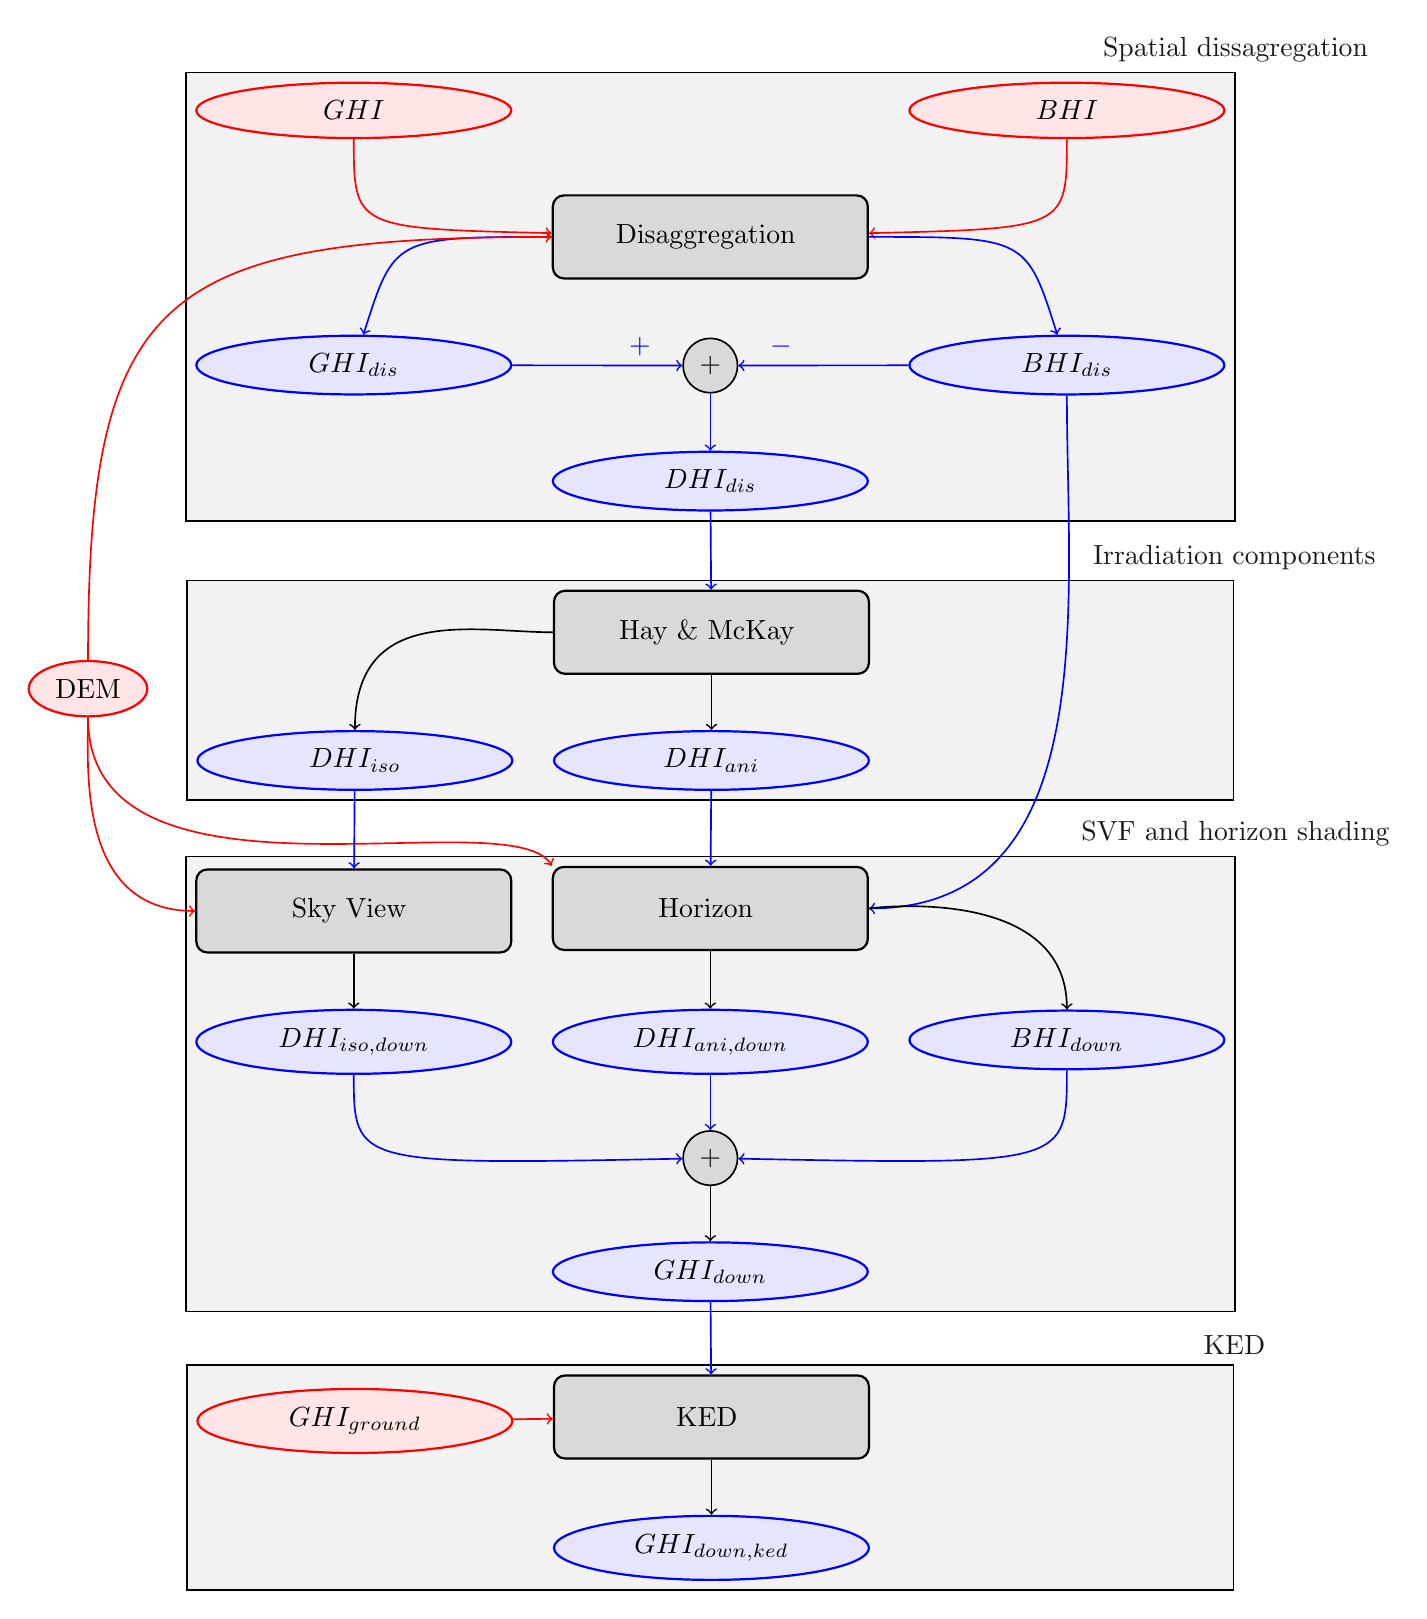
\begin{tikzpicture}[auto,
operation/.style={rectangle, rounded corners, draw=black, thick, fill=gray!30,
minimum height=3em, align=flush center, inner sep=1pt},
%
simple/.style={draw=black, circle, fill=gray!30},
%
source/.style ={draw=red, thick, ellipse, fill=red!10,
minimum height=2em},
%
result/.style ={draw=blue, thick, ellipse, fill=blue!10,
  minimum height=2em, }]

\tikzset{every path/.style={line width=.6pt}}

\begin{scope}
  \matrix [matrix of nodes, fill=gray!10, draw=black,column
  sep=5mm,row sep=7mm, minimum width=4cm] (disagM) {
    %%%%%%%%%%%%%%%%%%%%%%%%%%%%%%
    \node [source] (GHI) {$GHI$}; &
    \node {}; &
    \node [source] (BHI) {$BHI$}; \\
    %%%%%%%%%%%%%%%%%%%%%%%%%%%%%%
    \node {};& 
    \node [operation] (disag) { Disaggregation }; &  
    \node {}; \\
    %%%%%%%%%%%%%%%%%%%%%%%%%%%%%%
    \node [result] (GHId) { $GHI_{dis}$ }; &
    \node [simple, minimum width=2pt] (G-B) {$+$}; & 
    \node [result] (BHId) { $BHI_{dis}$ }; \\
    %%%%%%%%%%%%%%%%%%%%%%%%%%%%%%
    \node {}; & 
    \node [result] (DHId) {$DHI_{dis}$}; &
    \node {}; \\
  };
\end{scope}

\begin{scope}[yshift=-5cm]
  \matrix [matrix of nodes, fill=gray!10, draw=black, column
  sep=5mm,row sep=7mm, minimum width=4cm] (irradM) {
    %%%%%%%%%%%%%%%%%%%%%%%%%%%%%% 
    \node {}; &
    \node [operation] (Hay) { Hay \& McKay }; &
    \node {}; \\
    %%%%%%%%%%%%%%%%%%%%%%%%%%%%%%
    \node [result] (DHIiso) {$DHI_{iso}$}; &
    \node [result] (DHIani) {$DHI_{ani}$}; &
    \node {}; \\
    %%%%%%%%%%%%%%%%%%%%%%%%%%%%%%
  };
\end{scope}

\begin{scope}[yshift=-10cm]
  \matrix [matrix of nodes, fill=gray!10, draw=black,column
  sep=5mm,row sep=7mm, minimum width=4cm] (downM) {
    %%%%%%%%%%%%%%%%%%%%%%%%%%%%%% 
    \node [operation] (SVF) { Sky View }; &
    \node [operation] (Horizon) { Horizon }; & 
    \node (controlHorizon) {}; \\
    %%%%%%%%%%%%%%%%%%%%%%%%%%%%%% 
    \node [result] (DisoDown) { $DHI_{iso, down}$}; &
    \node [result] (DaniDown) { $DHI_{ani, down}$ }; &
    \node [result] (Bdown) { $BHI_{down}$}; \\
    %%%%%%%%%%%%%%%%%%%%%%%%%%%%%% 
    \node (controlSum1) {}; & 
    \node [simple, minimum width=2pt] (sum) {$+$}; & 
    \node (controlSum2) {}; \\
    %%%%%%%%%%%%%%%%%%%%%%%%%%%%%% 
    \node {}; & 
    \node [result] (Gdown) {$GHI_{down}$}; & 
    \node {}; \\
  };
\end{scope}

\begin{scope}[yshift=-15cm]
  \matrix [matrix of nodes, fill=gray!10, draw=black,column
  sep=5mm,row sep=7mm, minimum width=4cm] (kedM) {
    %%%%%%%%%%%%%%%%%%%%%%%%%%%%%% 
    \node [source] (ground) { $GHI_{ground}$}; &
    \node [operation] (KED) { KED }; &
    \node {}; \\
    %%%%%%%%%%%%%%%%%%%%%%%%%%%%%%
    \node {}; &
    \node [result] (GHIked) { $GHI_{down,ked}$}; &
    \node {}; \\
  };
\end{scope}


\begin{scope}
  \draw [->, red] (GHI) .. controls ++(-90:1.5) .. (disag);
  \draw [->, red] (BHI) .. controls ++(-90:1.5) .. (disag);
  \draw [->, blue] (disag.west) .. controls ++(180:2) .. (GHId);
  \draw [->, blue] (disag.east) .. controls ++(0:2) .. (BHId);
  \draw [->, blue] (GHId) -- node[near end] {$+$} (G-B); 
  \draw [->, blue] (BHId) -- node[above, near end] {$-$} (G-B); 
  \draw [->, blue] (G-B) -- (DHId); 
  %%%%%%%%%%%%%%%%%%%%%%%%%%%%%%
  \draw [->, blue] (DHId) -- (Hay); 
  \draw [->] (Hay) .. controls ++(180:3) and ++(90:2) .. (DHIiso); 
  \draw [->] (Hay) -- (DHIani); 
  %%%%%%%%%%%%%%%%%%%%%%%%%%%%%%
  \path (disagM.south west) -- (downM.north west) node[midway, source,
  xshift=-2cm] (DEM) {DEM};
  \draw [->, red] (DEM) .. controls ++(90:5) and ++ (180:5) .. (disag.west);
  \draw [->, red] (DEM) .. controls ++(-90:1) and ++(180:1.5) .. (SVF.west); 
  \draw [->, red] (DEM) .. controls ++(-90:3) and ++(120:1) .. (Horizon.north west);
  %%%%%%%%%%%%%%%%%%%%%%%%%%%%%%
  \draw [->, blue] (DHIiso) -- (SVF); 
  \draw [->, blue] (DHIani) -- (Horizon); 
  \draw [->, blue] (BHId) .. controls ++(-90:3) and ++(0:5) .. (Horizon); 
  \draw [->] (SVF) -- (DisoDown); 
  \draw [->] (Horizon) -- (DaniDown); 
  \draw [->] (Horizon) .. controls ++(0:2) and ++(90:2) .. (Bdown); 
  % \draw [->] (Horizon) .. controls (controlHorizon.south) .. (Bdown); 
  %%%%%%%%%%%%%%%%%%%%%%%%%%%%%%
  \draw [->, blue] (DisoDown) .. controls (controlSum1) .. (sum);
  \draw [->, blue] (Bdown) .. controls (controlSum2) .. (sum);
  \draw [->, blue] (DaniDown) -- (sum);
  %%%%%%%%%%%%%%%%%%%%%%%%%%%%%%
  \draw [->] (sum) -- (Gdown);
  \draw [->, blue] (Gdown) -- (KED);
  \draw [->, red] (ground) -- (KED);
  \draw [->] (KED) -- (GHIked);
  %%%%%%%%%%%%%%%%%%%%%%%%%%%%%%
  \node [color=black!90, above] at (irradM.north east) {Irradiation
    components};
  \node [color=black!90, above] at (disagM.north east) {Spatial
    dissagregation};
  \node [color=black!90, above] at (downM.north east) {SVF and horizon
    shading};
  \node [color=black!90, above] at (kedM.north east) {KED};
 
\end{scope}

\end{tikzpicture}

\end{document}